\subsection{Probabilistic Payments}
\label{sec:probabilisticpayments}

In traditional payment channels, two parties $A$ and $B$ lock some funds within a
smart contract, make transactions off-chain and only commit the aggregation
on-chain. Thus, a payment channel is bidirectional, which means both $A$ and $B$ can
send and receive transactions within the same payment channel. The HOPR protocol uses
unidirectional payment channels to implement bidirectional payment channel behavior, where one
payment channel is created from $A$ to $B$ and another from $B$ to $A$. The payment channel creator is
the sole owner of funds in the payment channel and the only one able to create
\textbf{tickets}, encapsulated funds which are described in detail in the
\nameref{sec:tickets} section. A payment channel created from party $A$ to party $B$ is
different from a payment channel created from party $B$ to party $A$.

$$A\rightarrow B \neq B\rightarrow A$$
\\~\\This separation reflects the directional nature of packets flowing through the
network. It also brings the advantage that each payment channel's logic is easier to verify.

\paragraph{Acknowledgements} are messages which allow every node to acknowledge
the processing of a packet to the previous node. This acknowledgement ($ACK$) contains
the cryptographic material needed to unlock the possible payout for the previous node.
Note that an acknowledgement is always sent to the previous node, and using
acknowledgments with vanilla payment channels results in accumulated incentives,
where the latest acknowledgement contains all previous incentives plus the
incentive for the most recent interaction, as explained below:

\begin{align}
value (ACK_n) &=\sum_{i=1}^nfee_{packet_i},
\end{align}
where $n$ is the total number of mixnet packets transformed.
\\~\\An issue arises when $B$ receives $ACK_n$ for $packet_n$ before sending
$packet_{n-1}$. At this point $B$ would have no incentive to process
$packet_{n-1}$ rather than $packet_{n}$. To avoid such false incentives, the HOPR
protocol utilizes probabilistic payments. A \textit{ticket} can be either a win
or a loss, determined based on some winning probability lower than 1. This means
nodes are incentivized to continue relaying packets, as they do not know which
tickets will result in a payout. From a node's perspective, each ticket has the same
value until it is claimed; therefore, the HOPR protocol encourages nodes to
claim tickets independently from each other.

\begin{align}
value ( ACK_i )  &  =value ( ACK_j ) \quad for \quad i,j\in \{1,n\}
\end{align}
\\~\\If we assume constant costs, there is no added value in pretending
packet loss or intentionally changing the order in which packets are processed.
On the contrary, a node would reduce its potential payouts if it were to forward
packets slowly or not at all.

\subsection{Payment Channel Management}
\label{sec:paymentchannelmanagement}

For node $A$ to transfer packets to node $B$, it must first open a payment channel. There are
four distinct payment channel states, represented in the following
scheme:

\begin{figure}[H]
    \centering
    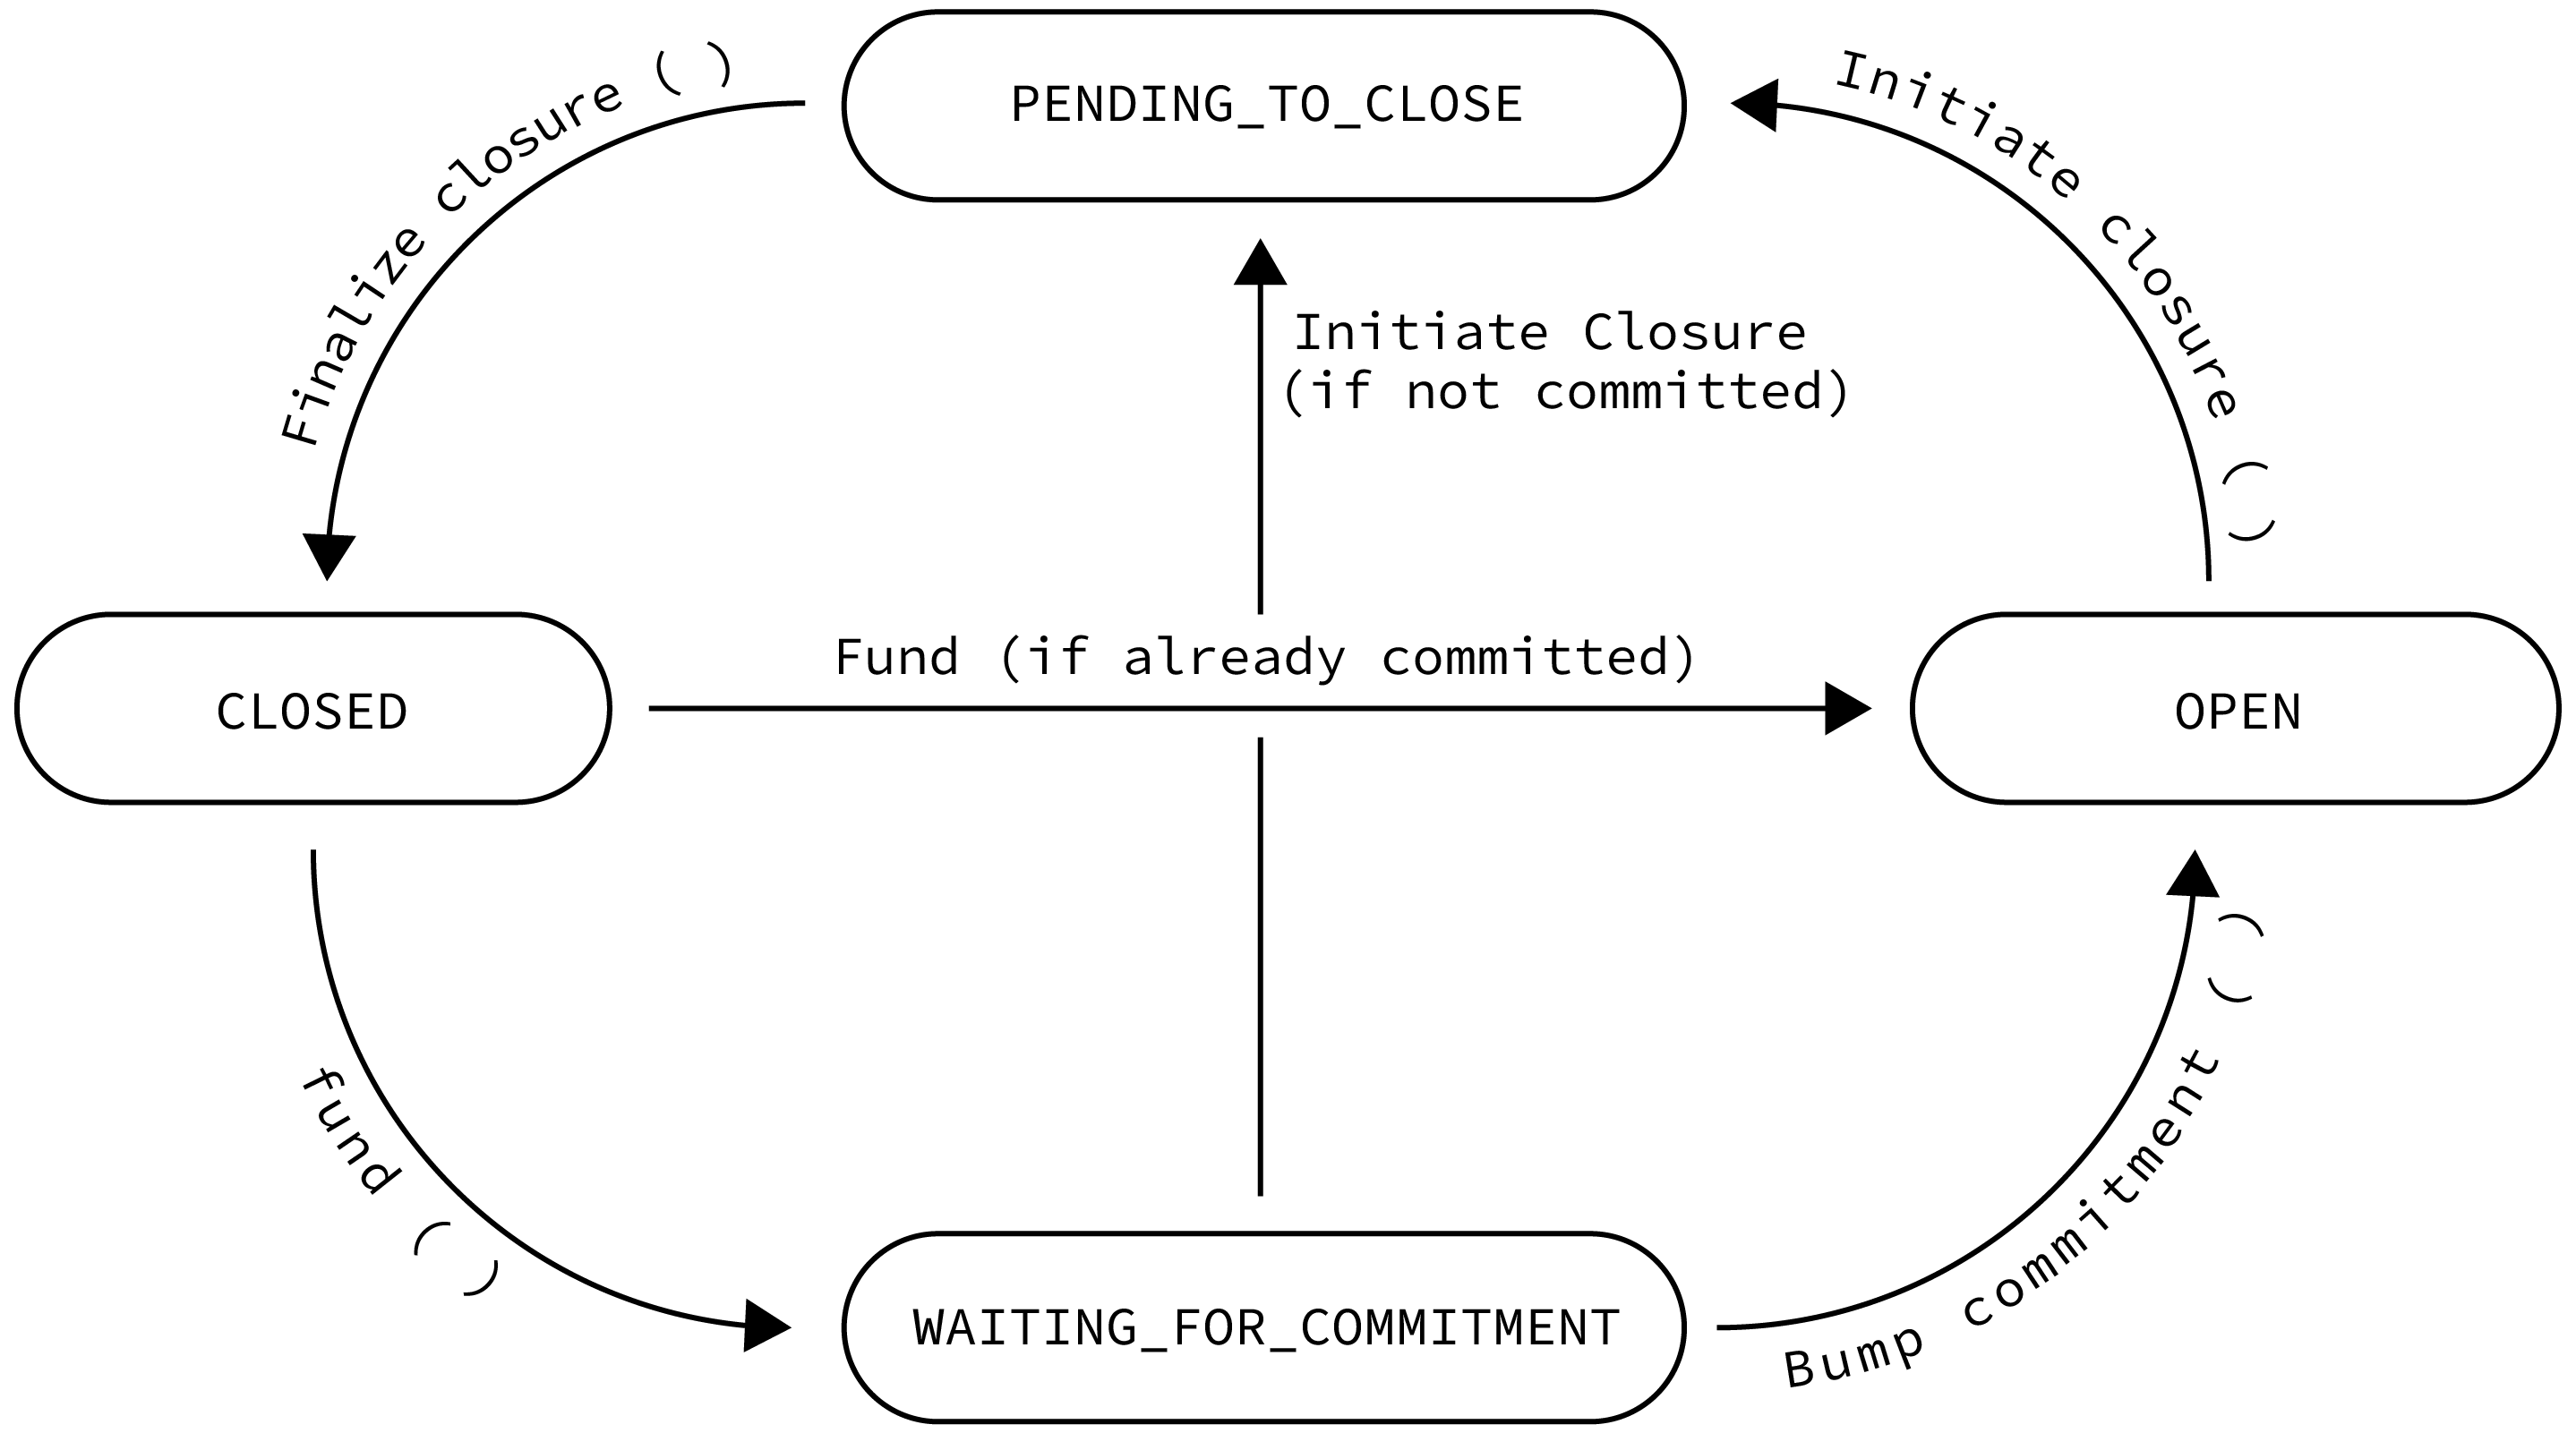
\includegraphics[width=9cm,height=9cm,keepaspectratio]{../yellowpaper/images/statesTransition.png}
    \label{fig:payment channel states}
    \caption{Payment channel states}
\end{figure}
Initially, each payment channel is \textit{Closed}. 

\paragraph{Opening a channel} Node $A$ can open a channel by transferring funds to
the payment channels contract \textit{HoprChannels} and including the following
\textit{userdata}:

$$[A: address, B: address, \lambda: uint8, \mu: uint8], \mu = 0,$$

where $\lambda$ is the amount to be staked by $A$. This call will trigger an on-chain event \textit{ChannelFunded}
and open a unidirectional payment channel from $A$ to $B$. The payment channel will start in state \textit{Waiting for commitment}. The destination address of the
payment channel must now set an on-chain commitment in order for the payment
channel between both parties to become \textit{Open}. This is done by $B$
calling the \textit{bumpChannel()} function to make a new set of commitments
towards this payment channel. This call will trigger an on-chain event
\textit{ChannelOpened} and bumps the ticket epoch to ensure tickets with the
previous epochs are invalidated. Every time the channel changes its state, an on-chain event \textit{ChannelUpdated} is emitted.

\paragraph{Redeeming tickets}
As long as the channel remains open, nodes can claim their incentives for
forwarding packets via tickets. Tickets are redeemed by dispatching a
\textit{redeemTicket()} call to an \textit{Open} payment channel.
\\~\\If $B$ tries to redeem a ticket from the channel $A\rightarrow B$ (spending
channel), but there is an open channel $B\rightarrow A$ (earning channel),
$B$'s rewards will be transferred to $B\rightarrow A$ (earning channel).
Otherwise, rewards will be sent directly to $B$.

\paragraph{Closing a channel}
Nodes can close a payment channel in order to access their previously staked
funds. Only the payment channel creator can initiate the process by calling
\textit{initiateChannelClosure()}. This changes the state to $Pending to close$
and triggers a grace period during which the destination node can redeem
any unredeemed tickets. Nodes should actively monitor blockchain events to
be aware of this payment channel state change.
\\~\\Once the grace period has elapsed, the payment channel creator can call
\textit{finalizeChannelClosure()} which changes the payment channel to
$Closed$. When a payment channel is closed, the remaining funds are automatically transferred
to the payment channel creator. The channel epoch increments, meaning any unredeemed tickets can no longer be redeemed.

\begin{comment}

\begin{figure}[H]
    \centering
    \begin{tikzpicture}[looseness=1,auto]
        \path (0,0) node (closed) [ellipse,draw] {$Closed$};
        \path (-1,-1)  node (commitment) [ellipse,draw,align=left] {$Waiting$\\$Commitment$};
        \path (5,0)  node (open) [ellipse,draw] {$Open$};
        \path (2.5,-1)  node (pending) [ellipse,draw,align=left] {$Pending$\\$Timeout$};

        \draw [->,draw](closed) to [bend left] node {\textsf{fund()}} (commitment);
        \draw [->,draw](commitment) to [bend left] node {\textsf{fund()}} (open);
        \draw [->,draw](open) to [bend left] node [align=center] {\textsf{initiateChannelClosure()}} (pending);
        \draw [->,draw](pending) to [bend left] node {\textsf{finalizeChannelClosure()}} (closed);

        \path[->] (open) edge [out=+120,in=+60,distance=2em,below] node [align=center,above] {\textsf{redeemTicket()}}  (open);
    \end{tikzpicture}
    \label{fig:channel workflow}
    \caption{Channel workflow}
\end{figure}
\end{comment}

\begin{comment}
  \draw [->,draw](commitment) to [bend left] node {\textsf{fund()}} (open);
    \draw [->,draw](open) to [bend left] node [align=center] {\textsf{initiateChannelClosure()}} (pending);
    \draw [->,draw](pending) to [bend left] node {\textsf{finalizeChannelClosure()}} (closed);  
\end{comment}
